\section{The Eternal Wedding}

Notwithstanding his idiosyncratic gnostic visions, \textbf{Miguel Serrano} can be astute in his estimations of Indian spirituality. During his pilgrimage to India, he visited the temples at Khajuraho. They are decorated with erotic sculptures, which seems rather strange in a country that is still shocked by an on-screen kiss. Serrano sees the erotic temples as a representation. He writes:

\begin{quotex}
The form of the temple is always the same. On the outer walls there are always hundreds of images reflecting war, life, death, love, procreation—in a word, Maya, or Illusion. But inside, in the most secret shrines, Siva meditates as a lingam. … the lingam symbolizes ecstatic concentration; it is the erect dorsal spine, along which the fire of the Serpent rises towards Samadhi. The interior Self or god remains unchanged in a profound dream, unaffected by what goes on externally, by its own creation which is reflected in the images on the outer walls of the temple. 

\end{quotex}
Serrano recognizes that this is all symbolism. He intuits the differences between the female and male figures in the sculptures. Of the former, he writes:

\begin{quotex}
Everywhere the female is fervent in love; she is wholly enveloped in the supreme passion, engaged in giving herself away. She searches for her lover, taking his head into her hands, enveloping him with her thighs, and bending and swinging her body. On her face is an expression of complete ecstasy, for she is engaged in making him wise and in perfecting him, while her body and her soul are totally lost in the act of giving. 

\end{quotex}
Note the contrast with the attitude of the male:

\begin{quotex}
The face of the male lover expresses no desire, but total absence. He is shown as though he were dreaming, with only one part of him remaining to sustain his lover, giving her protection and infinite tenderness. He appreciates her sacrifice and the pain she endures for his cause; he appreciates the technique which she has perfected in order to liberate him… she is the creation of the world. He is beyond her, he is beyond everything at the other end of the cord and he loves her with an infinite tenderness since he loves her as himself. He is immobile and abandoned. 

\end{quotex}
Serrano discusses the training of the men and women. In particular,

\begin{quotex}
The woman was not taught to satisfy man physically, but to touch his intimate centers, or chakras, and to impel him towards the Self. Thus the woman taught man to abandon her physically and to incorporate her spiritually within himself, so that he married not a woman but his own soul. 

\end{quotex}
Thus, for the man, Tantra has nothing to do with the pursuit of pleasure or sexual ecstasy as Evola mistakenly believed. Quite the contrary, as Serrano explains:

\begin{quotex}
The Tantric hero is forbidden to practice love passionately or compulsively. This is a rule permitted only to the woman. 

\end{quotex}
Serrano sums everything up:

\begin{quotex}
In all of this it must not be forgotten that what is important is the symbolic meaning or metaphor. Although written language and sculptured images may appear to be heavily overladen with sex, they are so only in appearance. On its highest plane, when it is practiced among the more sophisticated members of the cult, \emph{the Tantric ceremony is only a symbolic act}, for Maithuna [sexual union] occurs only with the body of the man. 

\end{quotex}
The union of opposites occurs progressively. Siva, the static principle, unites with Shakti, the dynamic principle. The feminine energy, Shakti, is Kundalini, the serpent; this unites with Atman, the achievement of Sunya or Emptiness.

Serrano points out that the practice of Tantra can lead to excesses, orgies, and aberrations, due to misunderstandings of the complex symbolism. However, he gets to the heart of the matter:

\begin{quotex}
The Tantrism of the Left Hand asserts that the road to liberation excludes nothing. It claims that self-denial and asceticism are absurd, since the Supreme Emptiness achieved in Sunya produces the same results, only more satisfactorily. Yet the Tantric method is the most difficult of all, for it demands continual vigilance over all parts of existence. It is the science of Siva, the Serpent. 

\end{quotex}

\begin{wrapfigure}{rt}{.3\textwidth}
 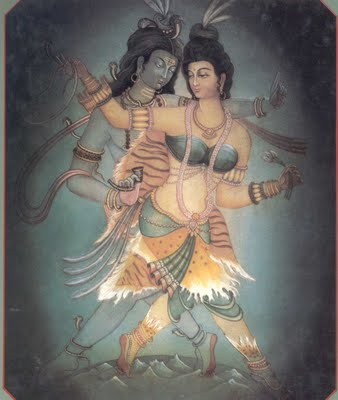
\includegraphics[scale=.3]{a20120304TheEternalWedding-img001.jpg}
\end{wrapfigure}
Is this at all clear? The Tantric path is easily confused with the pursuit of experiences that, despite their intensely pleasurable and ecstatic nature, are still no more than human, all too human. Ultimately, what is there to pursue since Atman, the unmoved mover, has no needs? There is nothing to seek, nothing to give up. All parts of existence provide us with the raw materials for transmutation, fuel for the awakening of the power of Shakti. The one thing necessary is to be ever vigilant, to be conscious of all that is moving, the images of Maya. That is to be as wise as the serpent.



\flrightit{Posted on 2012-03-04 by Cologero }

\begin{center}* * *\end{center}

\begin{footnotesize}\begin{sffamily}



\texttt{Matt on 2012-03-04 at 22:10 said: }

Yes, with all of Serrano's idiosyncrasies (the hidden nazi bases, ufo's, parallel universes etc.), he could be quite astute. He was also, to me at least, a great writer (even when his idiosyncrasies would reveal themselves and risk the coherency of his thought process). I found his writings to be very poetic. I read the Serpent of Paradise about 2 years ago at the bar/cafe at my university (ha I know, reading some Serrano at a university bar) after my classes were done for the week. I was so enthralled by it that I could not put it down and read it all the way through in that one sitting, never distracted by the chatter, hustle and bustle that went on all around me.

I think I'll revisit that book soon.


\end{sffamily}\end{footnotesize}
